\documentclass[a4paper]{article}

% Basic Packages
\usepackage[utf8]{inputenc}
\usepackage[T1]{fontenc}
\usepackage[a4paper,margin=1in]{geometry}
\usepackage{graphicx}
\usepackage{float} % for [H] figure placement
\usepackage{caption}
\usepackage{subcaption}
\usepackage{color}
\usepackage{amsmath, amssymb, amsfonts, amsthm}
\usepackage{mathrsfs}
\usepackage{algorithm, algpseudocode}
\usepackage{listings}
\usepackage{tikz}
\usepackage{fancyhdr}
\usepackage{titlesec}
\usepackage{natbib}
\usepackage{hyperref}
\usepackage[pages=all, color=black, position={current page.south}, placement=bottom, scale=1, opacity=1, vshift=5mm]{background}

% Bibliography Style
\bibliographystyle{mplainnat}
\usepackage[sort&compress,numbers,square]{natbib}

% Hyperref Setup
\hypersetup{
    unicode,
    pdfauthor={Gajjar Deep},
    pdftitle={Movie Recommendation System},
    pdfsubject={Recommender System using ML Algorithms},
    pdfkeywords={Recommendation System, KNN, GMM, Content-Based Filtering, ANN, SVM, Clustering},
    pdfproducer={LaTeX},
    pdfcreator={pdflatex}
}

% Theorem Environments
\theoremstyle{plain}
\newtheorem{theorem}{Theorem}
\newtheorem{definition}[theorem]{Definition}
\newtheorem{example}[theorem]{Example}
\newtheorem{remark}[theorem]{Remark}

% Listings setup
\definecolor{lightgray}{gray}{0.9}
\lstset{
  backgroundcolor=\color{lightgray},
  basicstyle=\ttfamily,
  frame=single,
  breaklines=true,
  postbreak=\mbox{\textcolor{red}{$\hookrightarrow$}\space}
}

\graphicspath{{fig/}}

% Title
\title{\textbf{Movie Recommendation System}}
\date{}

\begin{document}

\maketitle

\begin{abstract}
    
    \vspace{1em}
    \noindent\textbf{GitHub Repository:} \href{https://github.com/Levi477/Recommendation-Engine}
    {https://github.com/Levi477/Recommendation-Engine}
    
    \vspace{1em}
    \noindent\textbf{Website Link:}
    \href{https://recommendation-engine-eight.vercel.app}
    {https://recommendation-engine-eight.vercel.app}

    \vspace{1em}
    \noindent\textbf{Demo Video : }
    \href{https://youtu.be/9i2GlXGPWhg}
    {https://youtu.be/9i2GlXGPWhg}

    \vspace{1em}
    \noindent\textbf{Project Page Link : }
    \href{https://recommendation-engine-eight.vercel.app/project-page}
    {https://recommendation-engine-eight.vercel.app/project-page}
    
    \vspace{1em}
    \noindent\textbf{Resources : } 
    GeeksforGeeks for algorithms, Wikipedia for algorithms, IMDB for inspiration


    \end{abstract}

\tableofcontents

\newpage
\section{Introduction}
\label{sec:intro}

 This project implements a Movie Recommendation System using seven different machine learning techniques and \textbf{hosted backend on GCP (Google Cloud Platform ) VM}. It explores both content-based and user-based filtering through models like KNN, GMM, Clustering, SVM, and Neural Networks. The goal is to compare the performance and efficacy of these algorithms in recommending movies based on metadata or user interactions. 

\newpage
\section{Preprocessing and Feature Engineering}
\label{sec:preprocessing}

\subsection{Data Sources}
\begin{itemize}
    \item TMDB 5000 Movie Dataset (with metadata such as genres, keywords, overview, etc.)
    \item User interaction data simulated or gathered from user rating/feedback (if applicable)
\end{itemize}

\subsection{Cleaning and Normalization}
\begin{itemize}
    \item Removed duplicates and null entries.
    \item Converted genres and keywords from stringified JSON to usable lists.
    \item Normalized text by removing special characters, applying lowercasing, and tokenizing for text-based models.
\end{itemize}

\subsection{Feature Extraction}
\begin{itemize}
    \item \textbf{Title, Overview, Genres, Keywords, Cast, Crew}
    \item Used TF-IDF Vectorization on overview text for content similarity.
    \item Built a feature vector for each movie combining cast, crew, keywords, and genres.
\end{itemize}

\subsection{User-based Feature Engineering}
\begin{itemize}
    \item Mapping user interactions (likes, watches) into a binary matrix.
    \item Labeling movie IDs as indices for neural networks.
\end{itemize}

\subsection{Vectorization Techniques}
\begin{itemize}
    \item \textbf{TF-IDF}: Used for textual similarity from overviews.
    \item \textbf{CountVectorizer}: Used for bag-of-words models with keywords, cast, and genres.
    \item \textbf{PCA (Optional)}: Dimensionality reduction applied in some cases to reduce noise.
\end{itemize}

\begin{figure}[H]
    \centering
    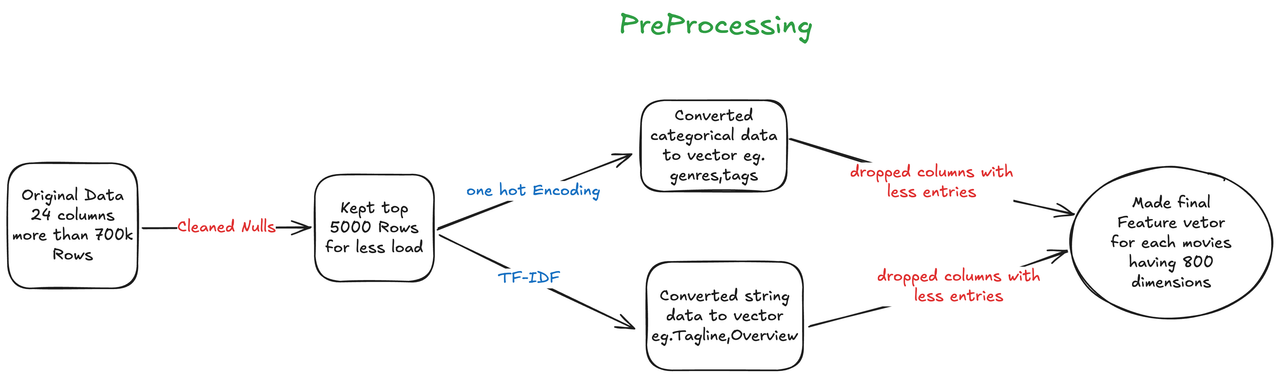
\includegraphics[width=\linewidth]{pre-processing.png}
    \caption{Feature Extraction Pipeline}
    \label{fig:pipeline}
\end{figure}

\newpage
\section{Approaches}

\subsection{K-Nearest Neighbors (KNN)}
\begin{figure}[H]
    \centering
    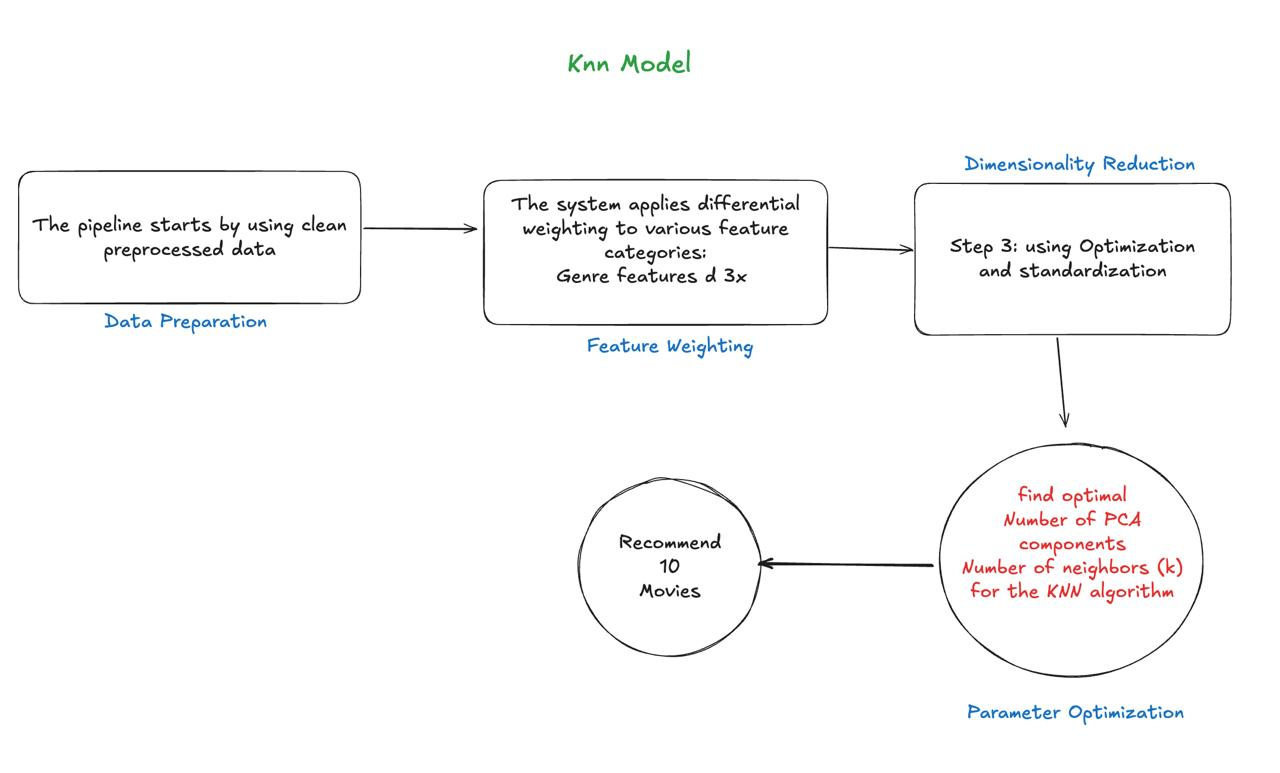
\includegraphics[width=\linewidth]{knn.jpg}
    \caption{KNN Similarity}
    \label{fig:knn}
\end{figure}

\begin{enumerate}
    \item We use \textbf{fuzzy matching} to find the closest matching movie title from the dataset, even if the input has typos or partial names. We select the match with a similarity score above a fixed threshold.

    \item Each feature (like genres, keywords) is given a different weight. For example, genres are given 3 times more weight than keywords. This ensures more important features have a stronger influence.

\begin{figure}[H]
    \centering
    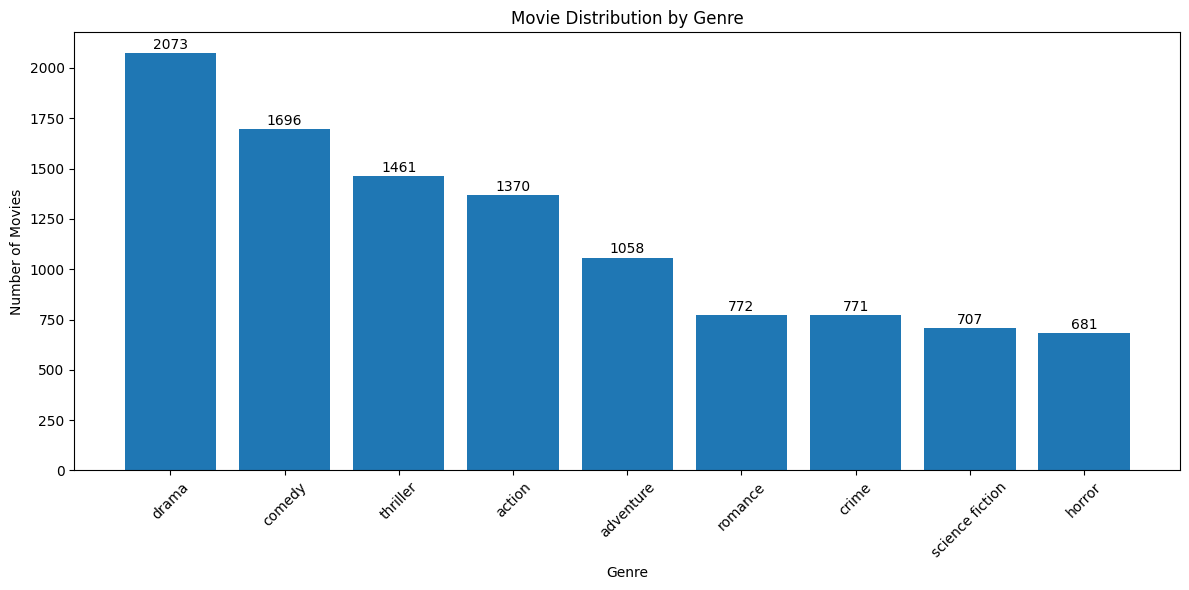
\includegraphics[width=\linewidth]{genre.png}
    \caption{Movie Distribution by Genre}
    \label{Figure 3}
\end{figure}

    \item PCA reduces the number of features while keeping most information. It helps speed up the system and reduces noise. We use a \textbf{cumulative explained variance} plot to decide the number of components needed to retain at least 95\% of the variance.

    \item KNN is used to find movies similar to the input movie.

    \textbf{Formula (Euclidean Distance):}
    \[
    d(p, q) = \sqrt{\sum_{i=1}^{n} (p_i - q_i)^2}
    \]
    Here, $p$ and $q$ are two movies represented as $n$-dimensional vectors. The smaller the distance $d(p, q)$, the more similar the movies are.

    

    \item To evaluate recommendations, we use the KNN algorithm to find the closest movies to the input movie in the feature space.
\end{enumerate}


\subsection{Gaussian Mixture Model (GMM)}
\begin{figure}[H]
    \centering
    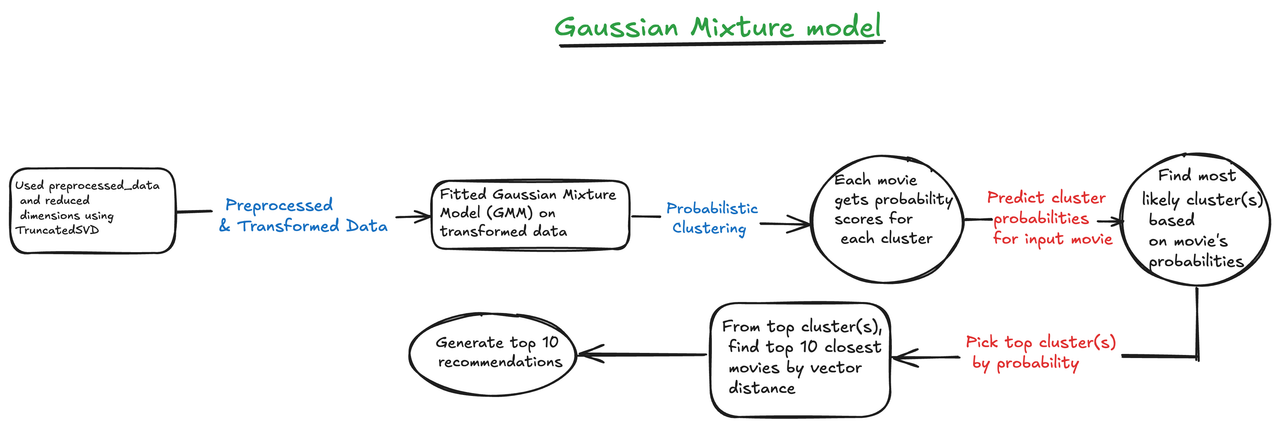
\includegraphics[width=\linewidth]{gmm.png}
    \caption{Gaussian Mixture Model Clustering}
    \label{fig:gmm}
\end{figure}

\[
P(x) = \sum_{k=1}^{K} \pi_k \mathcal{N}(x|\mu_k, \Sigma_k)
\]

\begin{enumerate}
    \item Use EM algorithm to find optimal parameters.
    \item Assign users to clusters based on probabilities.
    \item Recommend popular movies from that cluster.
\end{enumerate}


\subsection{K-Means Clustering }
\begin{figure}[H]
    \centering
    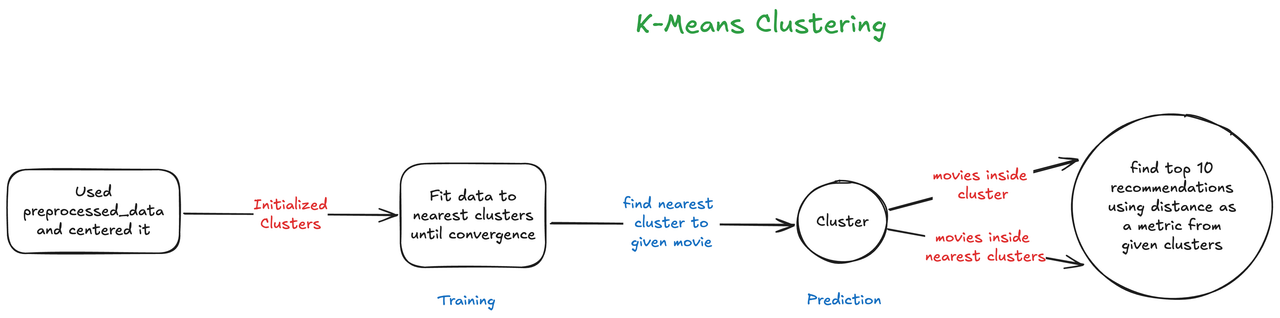
\includegraphics[width=\linewidth]{clustering.png}
    \caption{K-Means Clustering}
    \label{fig:clustering}
\end{figure}

\begin{enumerate}
    \item We first cleaned the dataset by removing irrelevant columns like \texttt{title} and \texttt{imdb\_id}, then normalized all numerical features using min-max scaling.

    \item \textbf{K-Means clustering} was applied on the preprocessed feature vectors to group similar movies. We chose $k = 7$ based on experimentation.

    \item Initial cluster centers were chosen using a variation of the K-Means++ initialization that considers the squared distance of each point from existing centers.

    \item In each iteration (epoch), every movie is assigned to the nearest cluster center. Then, the cluster centers are recalculated as the mean of all points within the cluster.

    \item The process repeats for 20 epochs or until convergence (when cluster centers stop changing).

    \item Once clustering is complete, recommendations can be made by selecting movies that belong to the same cluster as the input movie. If there are not enough options, the algorithm selects from the nearest cluster center.

    \item This method enables content-based recommendations using movie embeddings derived from metadata.

    \begin{figure}[H]
        \centering
        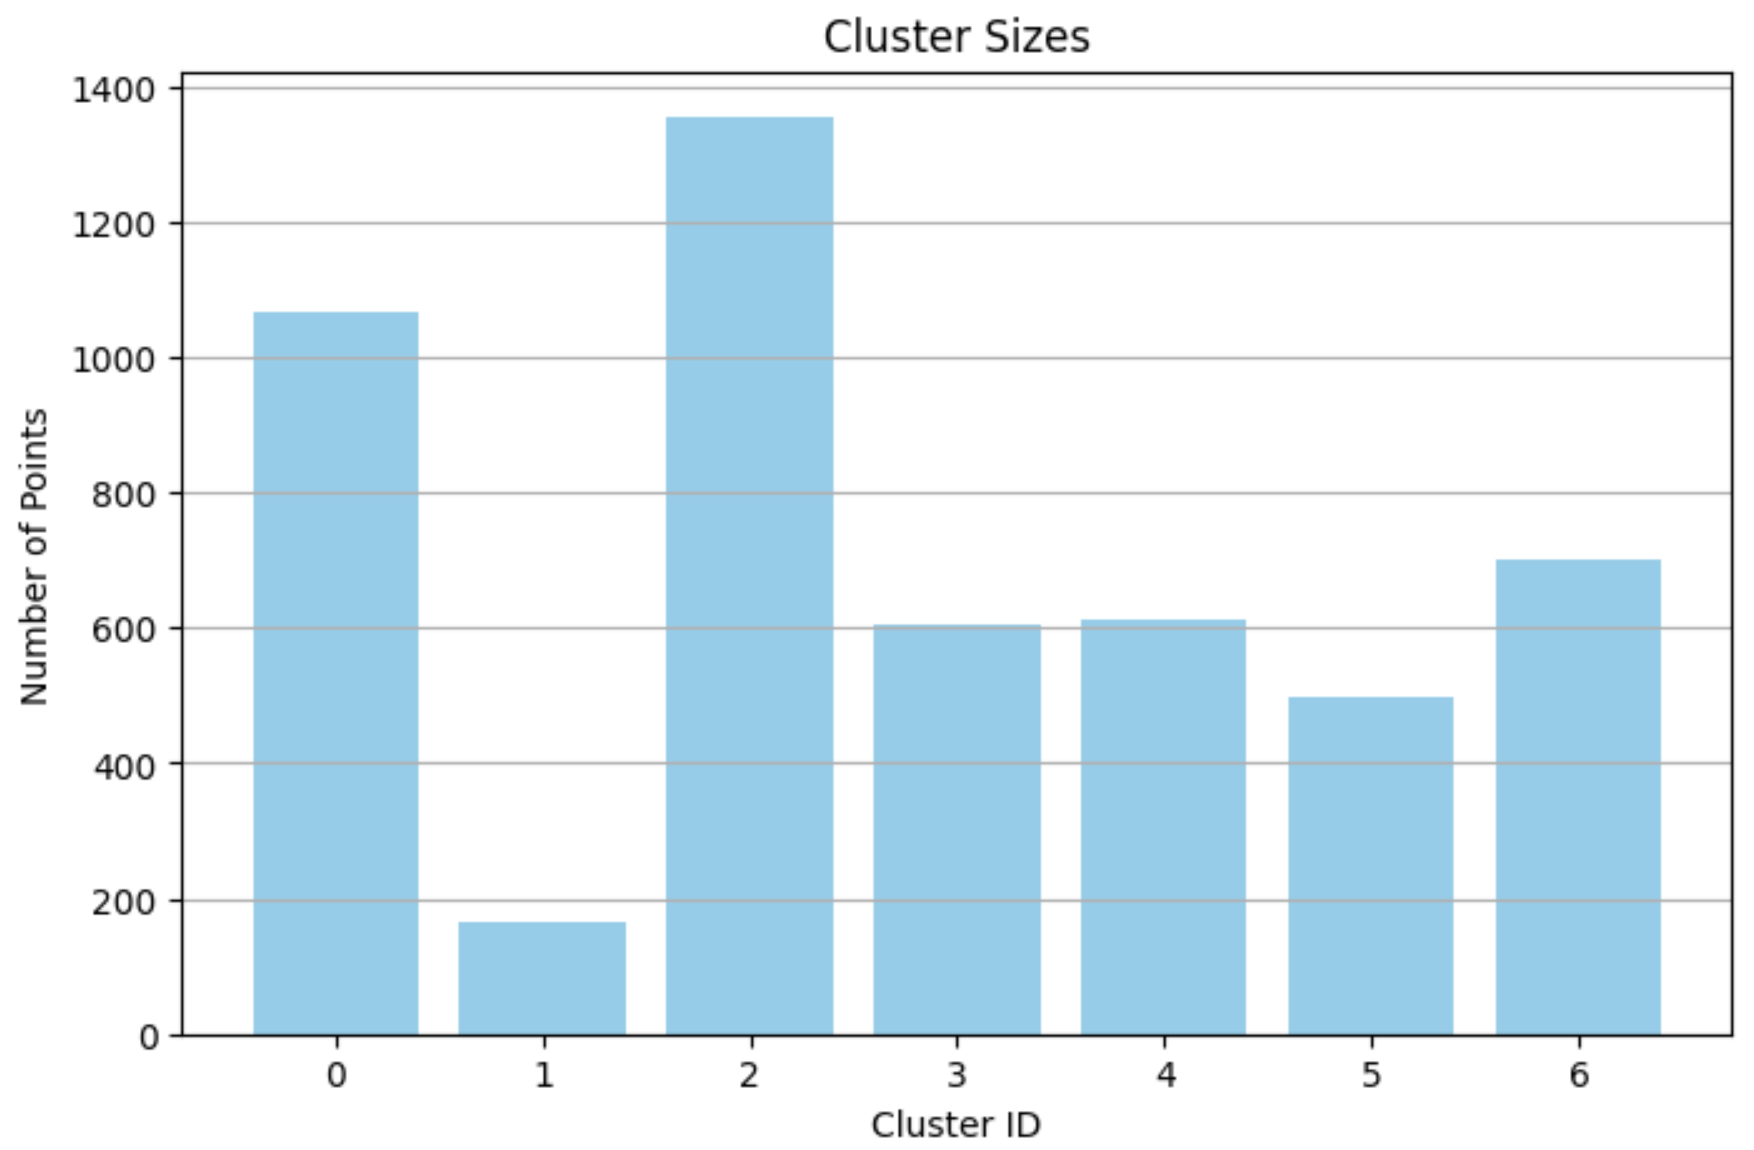
\includegraphics[width=\linewidth]{clustering1.png}
        \caption{Distribution of Movies Across K-Means Clusters}
        \label{fig:cluster_dist}
    \end{figure}

    \item 

    \textbf{Euclidean Distance Formula:}
    \[
    d(p, q) = \sqrt{\sum_{i=1}^{n} (p_i - q_i)^2}
    \]
    where $p$ and $q$ are $n$-dimensional feature vectors representing two movies.


    
\end{enumerate}


\subsection{Support Vector Machine (SVM)}
\begin{figure}[H]
    \centering
    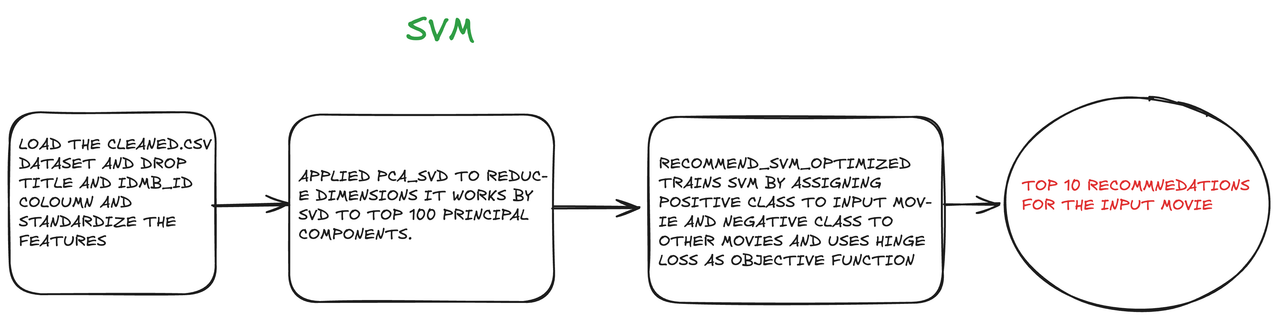
\includegraphics[width=\linewidth]{svm.png}
    \caption{Support Vector Machine}
    \label{fig:svm}
\end{figure}

\[
f(x) = \text w^T x + b
\]

\begin{enumerate}
    \item Load and Prepare Data(standardization).
    \item Do Dimensionality reduction using PCA using SVD(top 100 components).
    \item Learn a linear classifier that tries to separate the input movie from all others using a hinge-loss-based optimization (inspired by SVM).
    \item compute scores based on distance from hyperplane and returned  top movies.
\end{enumerate}

\subsection{Artificial Neural Network (ANN)}
\begin{figure}[H]
    \centering
    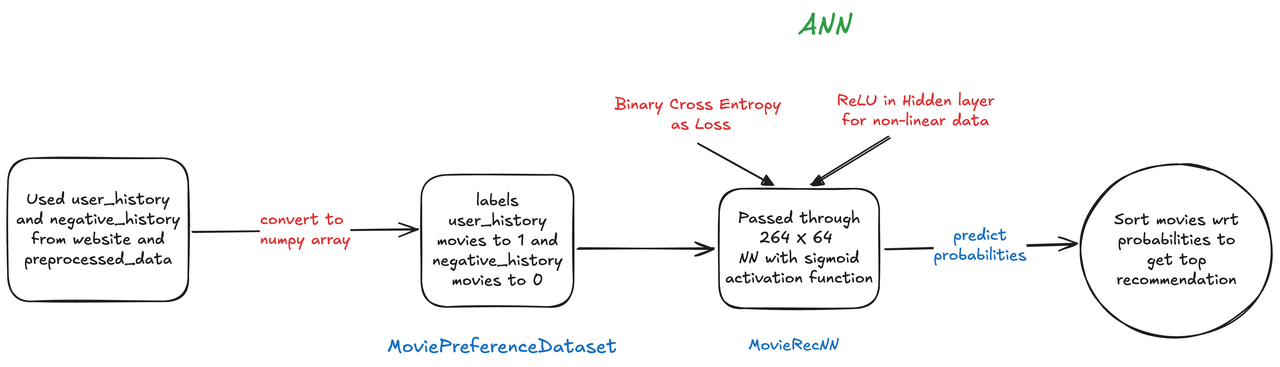
\includegraphics[width=\linewidth]{ann.png}
    \caption{Neural Network Architecture}
    \label{fig:ann}
\end{figure}

\[
\text{MSE} = \frac{1}{n} \sum_{i=1}^{n}(y_i - \hat{y}_i)^2
\]

\begin{enumerate}
    \item I uses User interactions (eg. CLicking the Movie) to filter out movies that user liked and disliked
    \item Make an array of positive-movies and negative-movies form above information to assign them label of 1 and 0 respectively
    \item Train model on given dataset of positive and negative movies.
    \item Use the weights gotten in previous step to predict movies with highest probability.
    \item Applied sigmoid activation function to get final probability
    \item Recommend movies with highest predicted scores.
\end{enumerate}

\subsection{Content-Based Filtering}
\begin{figure}[H]
    \centering
    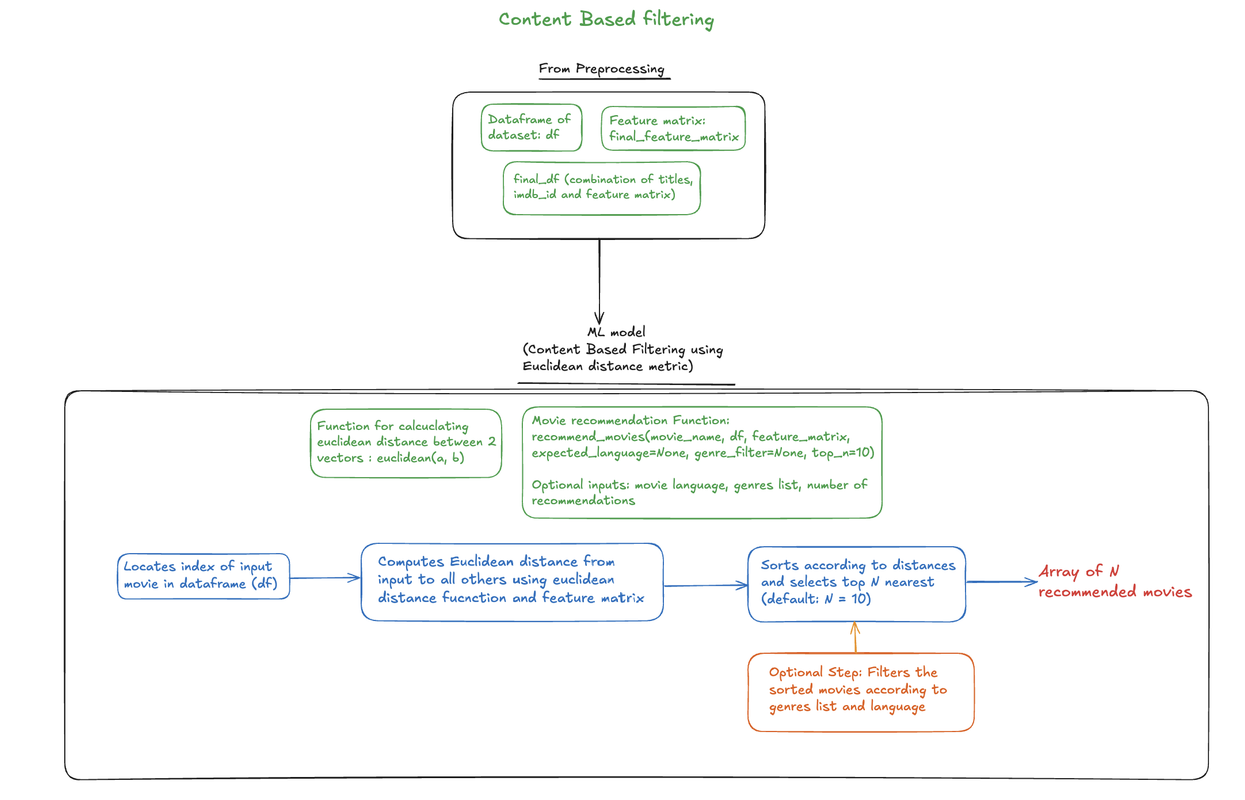
\includegraphics[width=\linewidth]{cbf.png}
    \caption{Content-Based Filtering}
    \label{fig:cbf}
\end{figure}
Euclidean distance:

\[
\text{euclidean}(a, b) =  \sqrt{\sum_{i=1}^{n} (a_i - b_i)^2}
\]

\begin{enumerate}
    \item Take the feature matrix (created using TF-IDF and encoding techniques) and calculate the similarities between selected and other movies.
    \item Sort the movies according to similarities (euclidean distances).
    \item Recommend the top N similar movies to user's selected movie.
\end{enumerate}
\begin{figure}[H]
    \centering
    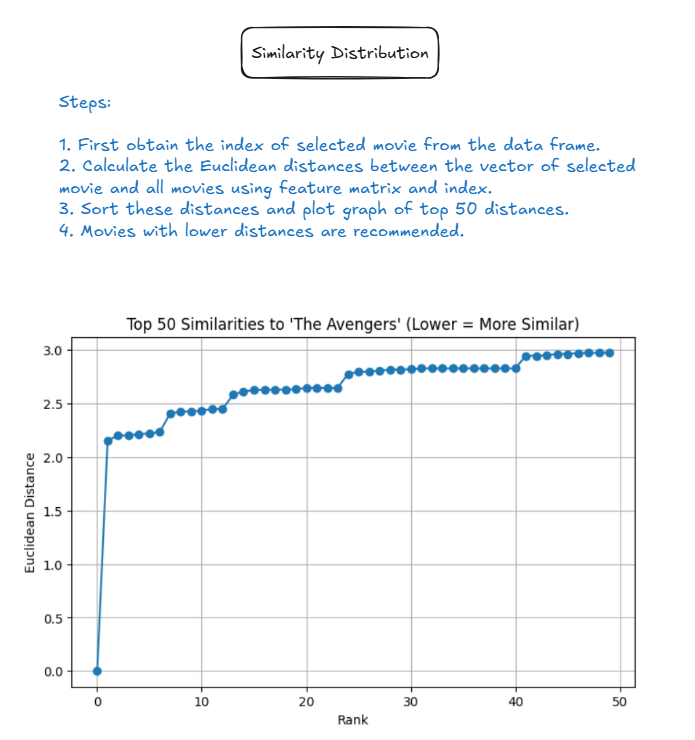
\includegraphics[width=\linewidth]{cbf_vis1.png}
    \caption{Content-Based Filtering - Similarity Scores}
    \label{fig:cbf}
\end{figure}
\subsection{Bayesian Recommendation}
\subsubsection{Traditional approach}
\begin{figure}[H]
    \centering
    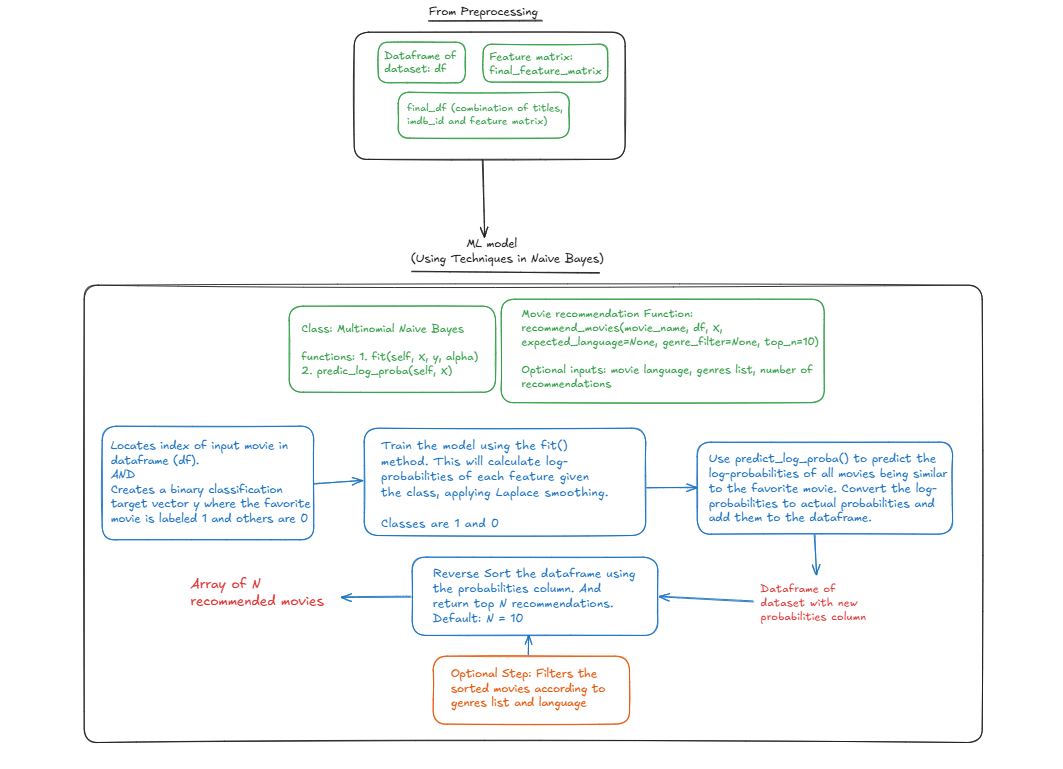
\includegraphics[width=\linewidth]{bayestrad.png}
    \caption{Bayesian Model: Similar to Traditional Method}
    \label{fig:bayesian}
\end{figure}

Formula:
\[
log P(c \mid \mathbf{x}) = log P(c) + \sum_{i=1}^{n} x_i \cdot log P(w_i \mid c)
\]
\newline
\begin{enumerate}
    \item In this method, we create two classes, 1 for selected movie and 0 for all other remaining movies
    \item  Then we calculate the prior log probability for each class ( log P(c) ) and log probabilities of the features/words for that class (log P(wi | c)) along with Laplace smoothing.
    \item After this, we iterate through all movies and calculate the log probabilities of these movies for the given classes according to formula. 
    \item Then top N movies with high probabilities for class 1 are recommended \end{enumerate}
\begin{figure}
    \centering
    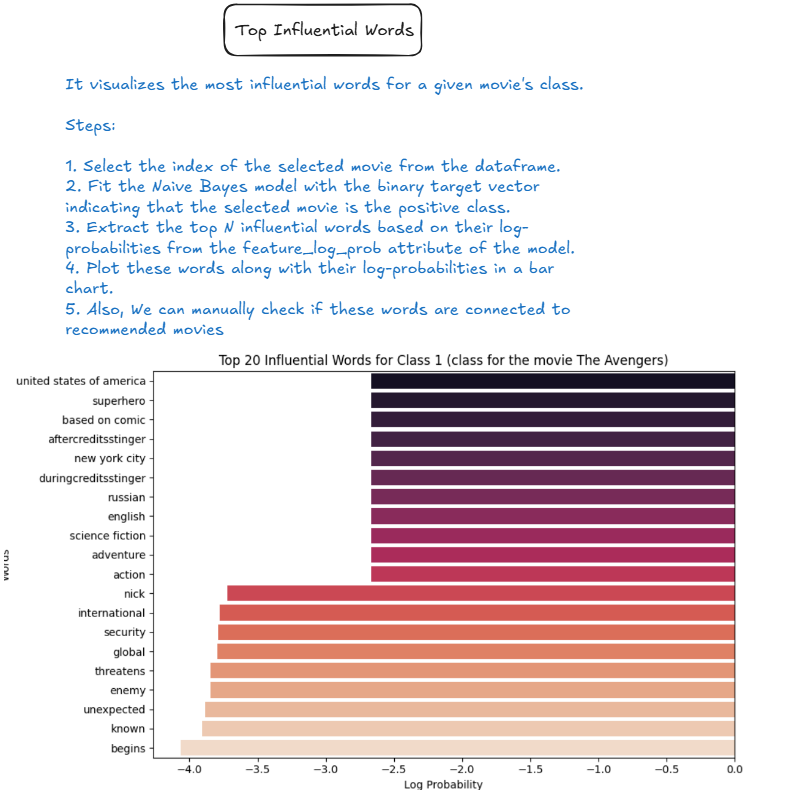
\includegraphics[width=\linewidth]{baytrad2.png}
    \caption{Top Influential words}
    \label{fig:enter-label}
\end{figure}


\subsubsection{Modified approach}
\begin{figure}[H]
    \centering
    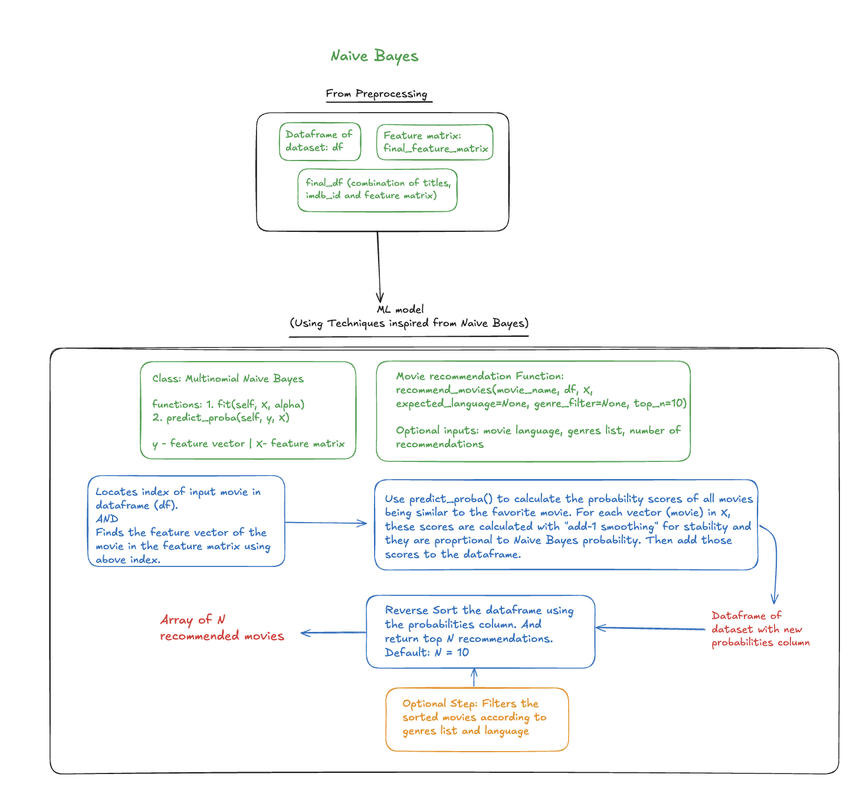
\includegraphics[width=\linewidth]{bay.png}
    \caption{Bayesian Recommendation Model}
    \label{fig:bayesian}
\end{figure}

Formula:
\[
Score(d_i, q) \propto \prod_{j=1}^{|V|} (q_j + 1)^{d_{ij}}
\]
\newline
\begin{enumerate}
    \item Instead of traditional classification method, we compute the \textbf{likelihood of other movies} being generated by the input movie’s word distribution. 
    \item First, we take the selected movie's feature vector. Then we iterate through all of the movies vectors and compute the similarity scores (probability scores) for each movie using the above formula.
    \item In the formula, q is selected movie's feature vector and di is any movie's feature vector from the list of all movies.
    \item Recommend the top N movies with highest probability scores.
\end{enumerate}
\newpage
\section{Analysis and Results}
\label{sec:results}

After implementing and evaluating the seven different recommendation techniques, we compared their output,likliehood or their clusters.

\subsection{K-Nearest Neighbors (KNN)}
PCA reduces the number of features while keeping most information. It helps speed up the system and reduces noise. We use a \textbf{cumulative explained variance} plot to decide the number of components needed to retain at least 95\% of the variance. give title for this graph
  \begin{figure}[H]
      \centering
      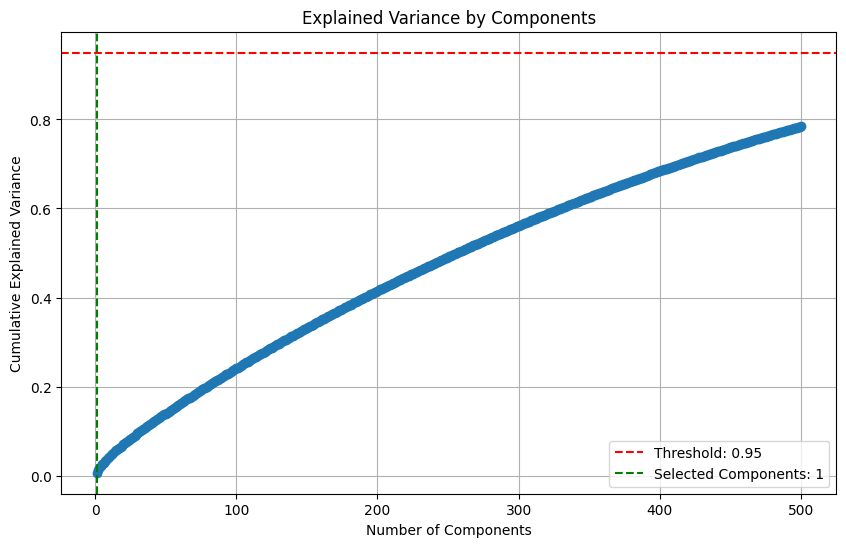
\includegraphics[width=\linewidth]{variance.png}
      \caption{Variance}
      \label{fig:enter-label}
  \end{figure}

\subsection{K-Means Clustering}
    \begin{figure}[H]
        \centering
        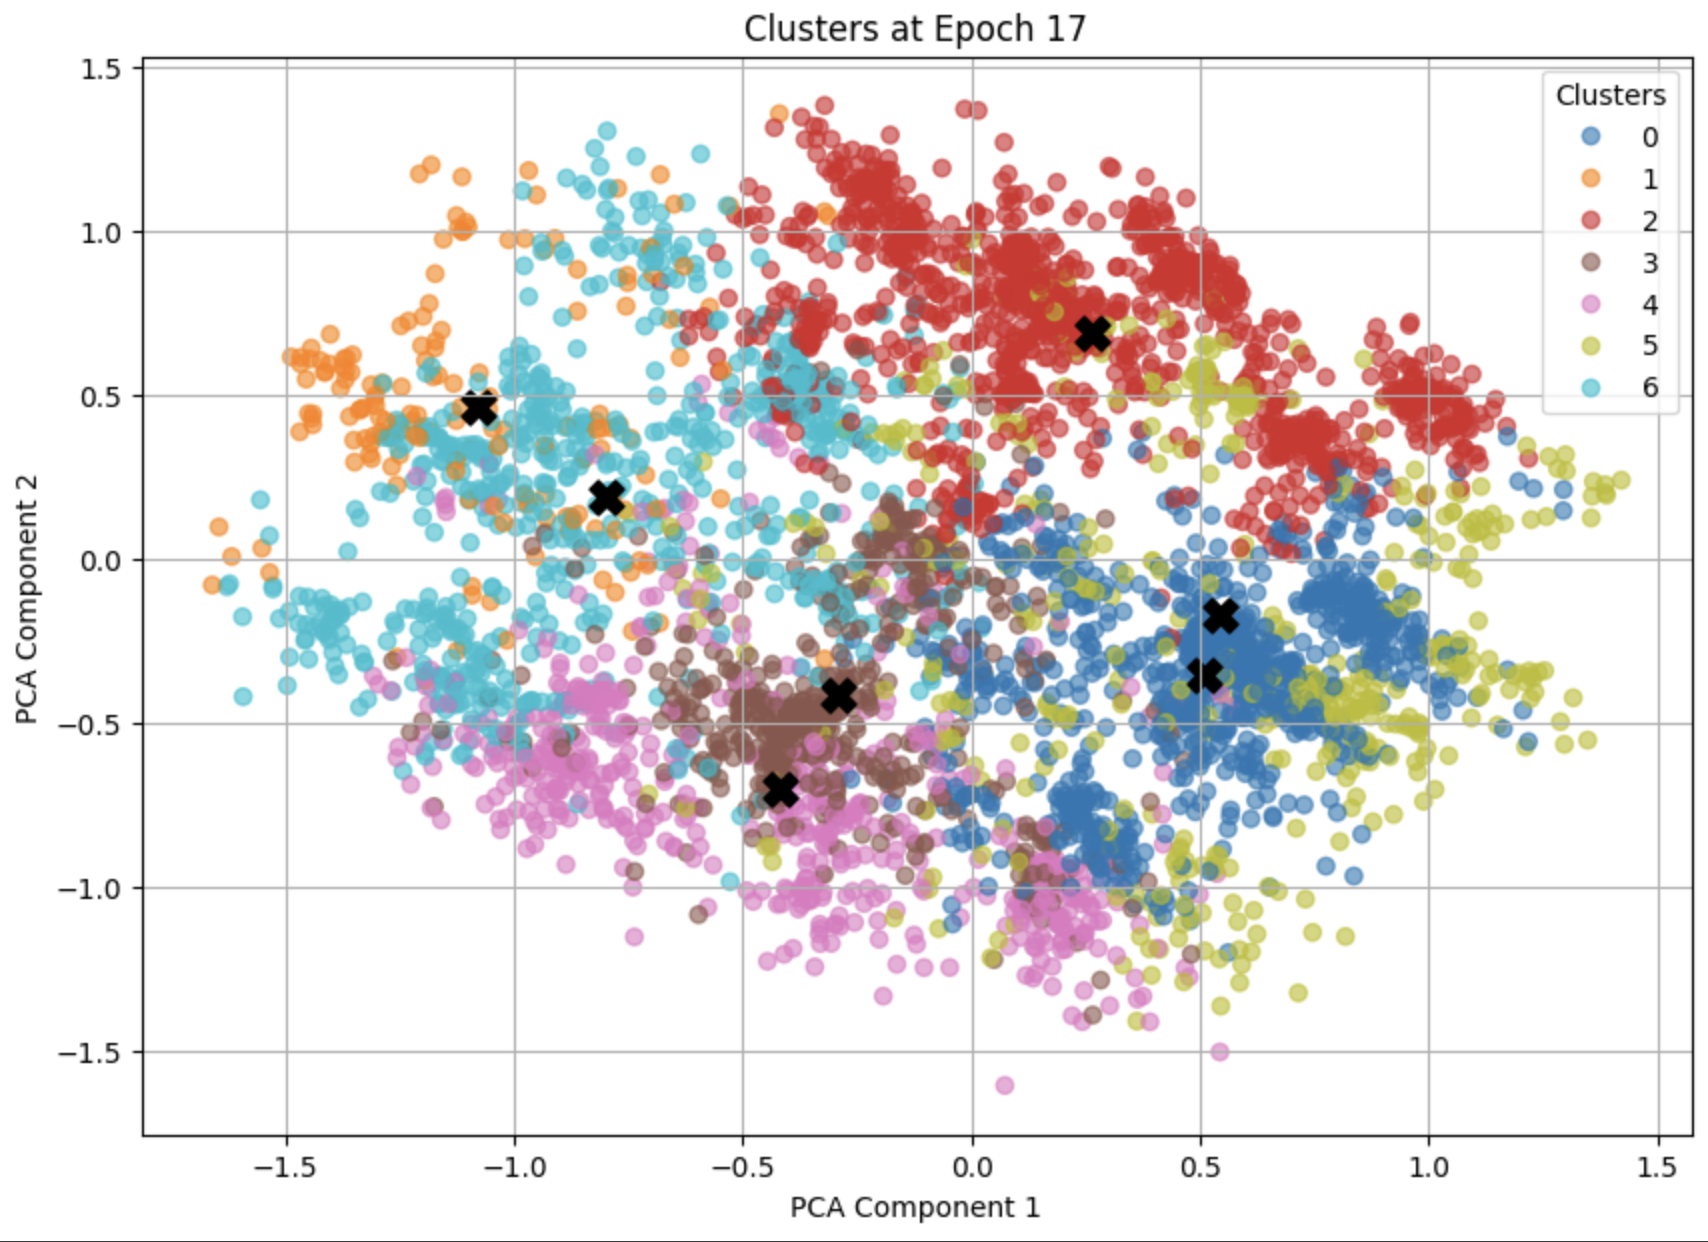
\includegraphics[width=\linewidth]{clustering2.png}
        \caption{Distribution of Movies Across K-Means Clusters in reduced dimension}
        \label{fig:cluster_dist}
    \end{figure}

\subsection{Content-Based Filtering}

\subsubsection{Genre Importance Matrix}
It visualizes the similarity in the genres of selected movie and recommended movies.
\begin{figure}[H]
    \centering
    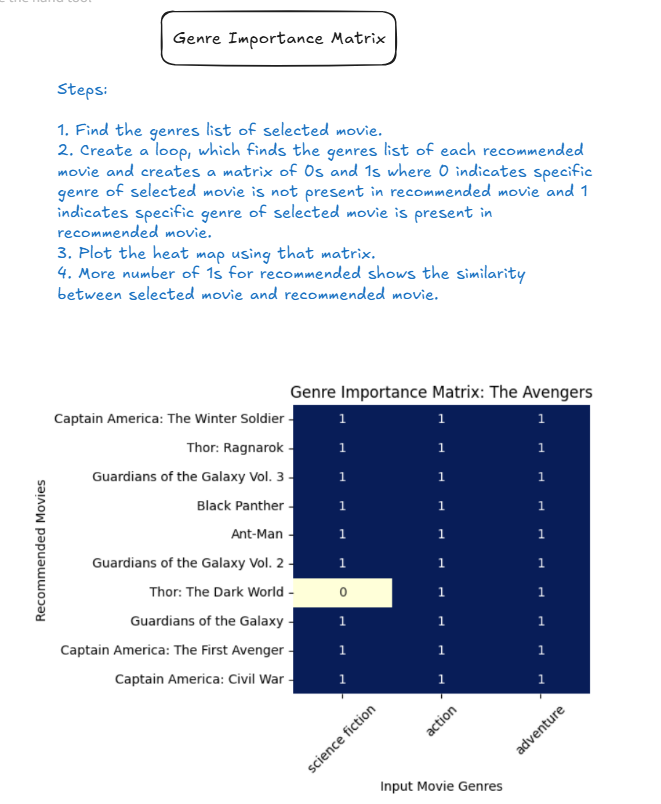
\includegraphics[width=\linewidth]{cbf_vis2.png}
    \caption{Content-Based Filtering - Genre Importance Matrix}
    \label{fig:cbf}
\end{figure}

\subsection{Bayesian Techniques}
\subsubsection{Traditional approach:}
\begin{figure}[H]
    \centering
    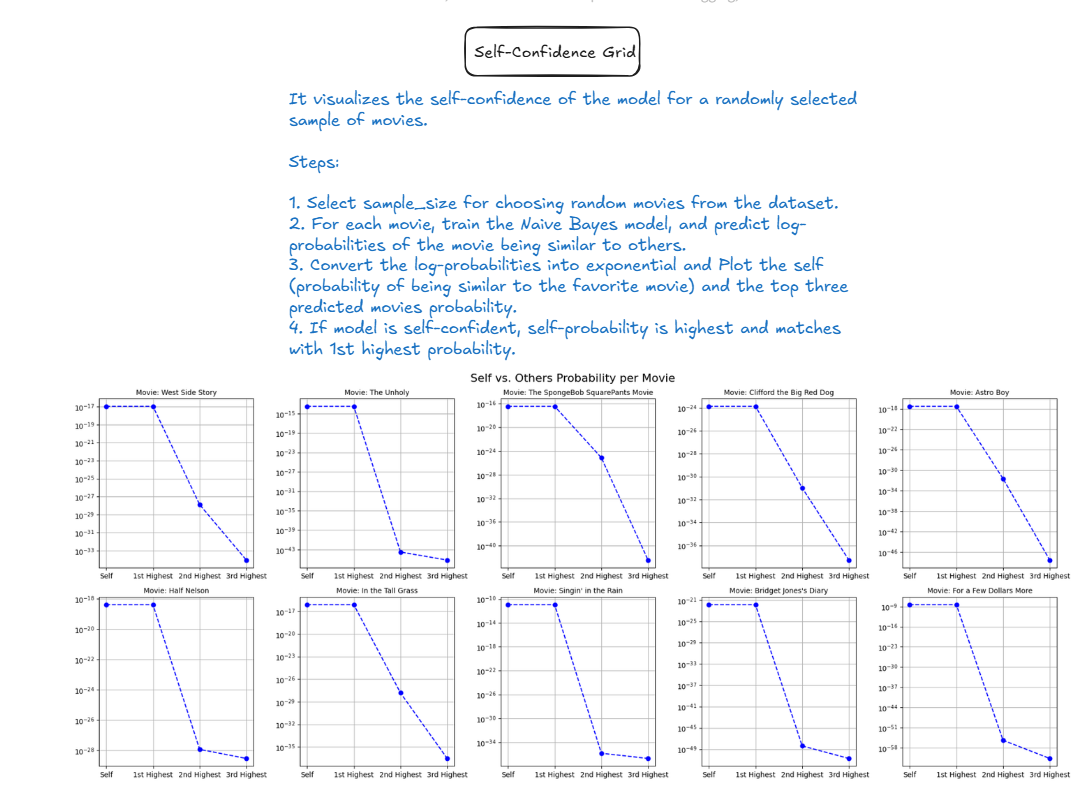
\includegraphics[width=\linewidth]{baytrad1.png}
    \caption{Bayesian Techniques- traditional approach : Self-Confidence Grid}
    \label{fig:cbf}
\end{figure}

\subsubsection{Modified Approach:}
It is observed that Self-importance grid is similar to traditional approach but improvement is made in better recommendations.
\begin{figure}
    \centering
    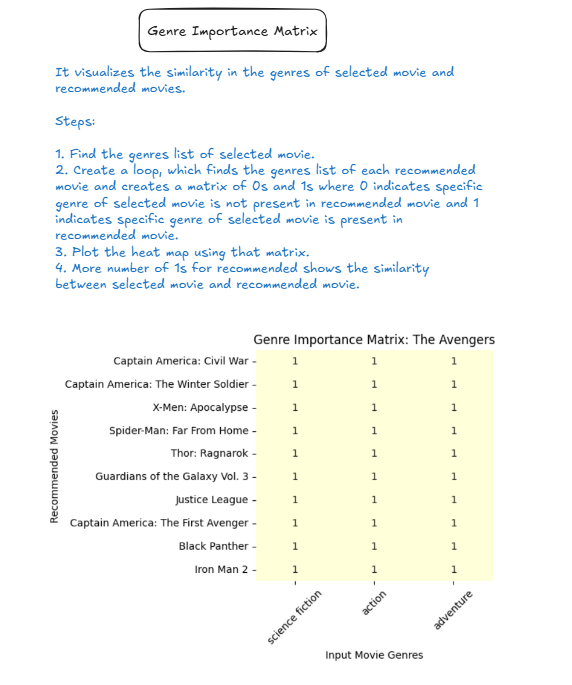
\includegraphics[width=1\linewidth]{baymod1.png}
    \caption{Bayesian techniques - modified approach: Genre Importance Matrix}
    \label{fig:enter-label}
\end{figure}
\newpage
\section{Summary of Model Performance}
\begin{table}[H]
    \centering
    \begin{tabular}{|l|c|c|c|c|}
        \hline
        \textbf{Model} & \textbf{Accuracy} & \textbf{Personalization} & \textbf{Complexity} & \textbf{Remarks} \\
        \hline
        KNN & High & Medium & Low & Fast, interpretable \\
        GMM & Medium & Low & Medium & Good for group-based suggestions \\
        Content-Based & Medium & High & Medium & Cold-start friendly \\
        K-Means & Medium & Medium & Low & Useful for segmentation \\
        SVM & High & Medium & High & Effective with labeled data \\
        ANN & Very High & Very High & Very High & Excellent accuracy, needs large dataset \\
        Bayesian & Medium & High & Medium & Probabilistic, robust \\
        \hline
    \end{tabular}
    \caption{Comparative Analysis of Recommendation Models}
    \label{tab:comparison}
\end{table}

\subsection{Observations}
\begin{itemize}
    \item \textbf{ANN} gave the best overall performance in terms of personalization and accuracy, but requires heavy computational resources.
    \item \textbf{KNN} was fast, interpretable, and reliable for collaborative filtering scenarios.
    \item \textbf{Content-Based Filtering} excelled in personalizing suggestions based on movie features.
    \item \textbf{GMM} is accurate and has great performance.
    \item \textbf{Clustering methods} like GMM and K-Means worked well for grouping similar user preferences but sometimes lacked precision 
    \item \textbf{SVM} was effective in classification-based recommendation settings but scaled poorly for large datasets.
    \item \textbf{Bayesian Methods} provided explainable and consistent recommendations.
\end{itemize}

\subsection{Conclusion}
There is no universal best algorithm—each has its advantages depending on the specific use-case, data availability, and user behavior. In practice, hybrid models that combine collaborative, content-based, and neural network approaches often yield the most robust performance.
There is no universal best algorithm—each has its advantages depending on the specific use-case, data availability, and user behavior. In practice, hybrid models that combine collaborative, content-based, and neural network approaches often yield the most robust performance.

\section{Contributions}
\paragraph{Deep Gajjar (B23EE1014) : }
Data Cleaning/Preprocessing and Vectorization, Implemented ANN (Artificial Neural Network) algorithm
\paragraph{Abhyudaya Tiwari (B23CS1085) : }
Implemented KNN algorithm,Created backend for all the models and Deployed on GCP(Google Cloud Platform)
\paragraph{Neeraj Kumar (B23CS1044) : }
Implemented K-Means Clustring Algorithm, Created Frontend Website for the project
\paragraph{Pawar Yuvraj Pramod (B23CS1051): }
Implemented Bayesian ( Both Traditional and Modified) and Content Based Filtering models
\paragraph{Bhavya Uchhat (B23CS1074) : }
Implemented GMM(Gausian Mixtureing Model) algorithm for Reocmmendation
\paragraph{Patil Sanskar (B23CS1050) : }
Implemented SVM(Scalable Vector Machine) algorithm for Recommendation
\end{document}